% Gemini theme
% See: https://rev.cs.uchicago.edu/k4rtik/gemini-uccs
% A fork of https://github.com/anishathalye/gemini

\documentclass[final]{beamer}

% ====================
% Packages
% ====================

\usepackage[T1]{fontenc}
\usepackage{lmodern}
\usepackage[size=custom,width=120,height=72,scale=1.0]{beamerposter}
\usetheme{gemini}
% \usecolortheme{uchicago}
\usecolortheme{stanford}
\usepackage{graphicx}
\usepackage{booktabs}
\usepackage{tikz}
\usepackage{pgfplots}
\pgfplotsset{compat=1.17}

% ====================
% Lengths
% ====================

% If you have N columns, choose \sepwidth and \colwidth such that
% (N+1)*\sepwidth + N*\colwidth = \paperwidth
\newlength{\sepwidth}
\newlength{\colwidth}
\setlength{\sepwidth}{0.025\paperwidth}
\setlength{\colwidth}{0.3\paperwidth}

\newcommand{\separatorcolumn}{\begin{column}{\sepwidth}\end{column}}


\title{Learning Neural Orientation Field for Volumetric Hair Reconstruction}


\author{Fangjun Zhou \inst{1} \and Zhenyu Zhang \inst{1} \and Weiran Xu \inst{1}}

\institute[shortinst]{\inst{1} Computer Science, Stanford}

% ====================
% Footer (optional)
% ====================

\footercontent{
  % \href{rylanschaeffer.github.io}{rylanschaeffer.github.io} \hfill
  % NeurIPS 2021 Workshop: Metacognition in the Age of AI \hfill
  % \href{mailto:rylanschaeffer@gmail.com}{rylanschaeffer@gmail.com}
  }
% (can be left out to remove footer)

% ====================
% Logo (optional)
% ====================

% use this to include logos on the left and/or right side of the header:
% \logoright{\includegraphics[height=7cm]{logos/cs-logo-maroon.png}}
% \logoleft{\includegraphics[height=7cm]{logos/cs-logo-maroon.png}}

% ====================
% Body
% ====================

\begin{document}

% This adds the Logos on the top left and top right
\addtobeamertemplate{headline}{}
{
    \begin{tikzpicture}[remember picture,overlay]
    %   \node [anchor=north west, inner sep=3cm] at ([xshift=0.0cm,yshift=1.0cm]current page.north west)
    %   {\includegraphics[height=5.0cm]{stanford_logos/Stanford-CS.png}}; % uc-logo-white.eps
      \node [anchor=north east, inner sep=3cm] at ([xshift=0.0cm,yshift=2.5cm]current page.north east)
      {
\includegraphics[height=7.0cm]{stanford_logos/Block_S_2_color.png}};
    \end{tikzpicture}
}

\begin{frame}[t]

\begin{columns}[t]

\separatorcolumn

\begin{column}{\colwidth}

  \begin{block}{Introduction}

    Reconstructing human hair is one of the most challenging yet critical process in rendering photorealistic digital human. In this work, we propose a new method capturing the hair structure by learning a 3D orientation field from $\mathbb{R}^{3} \rightarrow \mathbb{R}^{2}$ representing the hair growing direction. Given a set of portraits with annotated hair orientation, our method effectively reconstructs hair orientation from unseen angles with high-resolution and robustness.

  \end{block}

  \begin{block}{Data}
  
  The dataset used by this project is generated by a Blender geometry node-based hair system demo file. We render the model from multiple viewing angles and exported the camera intrinsics and extrinsics for later use.

    Our training set consists of 128 instances and our test set consists of 16 instances, all rendered from the same model but with different camera poses.

    \begin{figure}[h]
        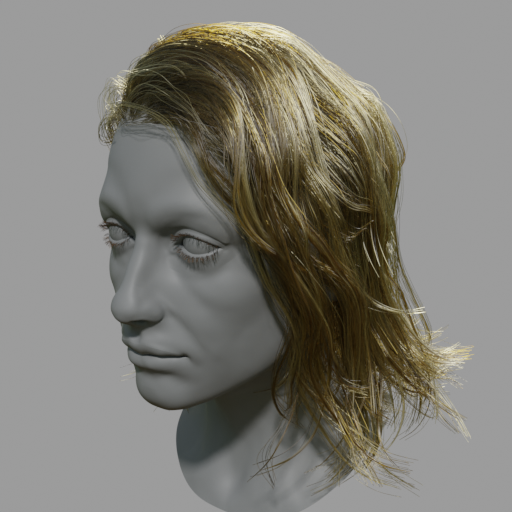
\includegraphics[width=0.2\textwidth]{project-final-paper/images/dataset/0009_rendered.png}
        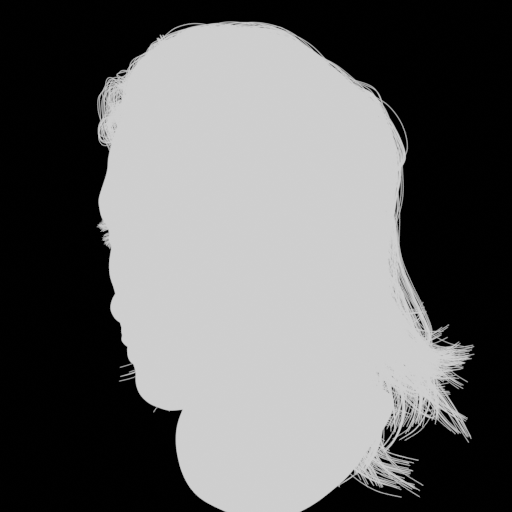
\includegraphics[width=0.2\textwidth]{project-final-paper/images/dataset/0009_bodymask.png}
        \centering
        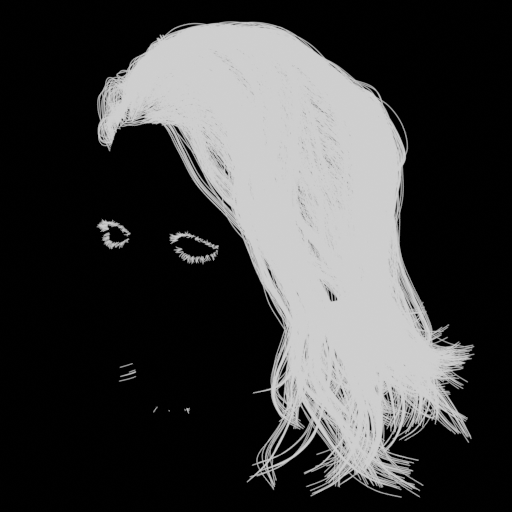
\includegraphics[width=0.2\textwidth]{project-final-paper/images/dataset/0009_hairmask.png}
        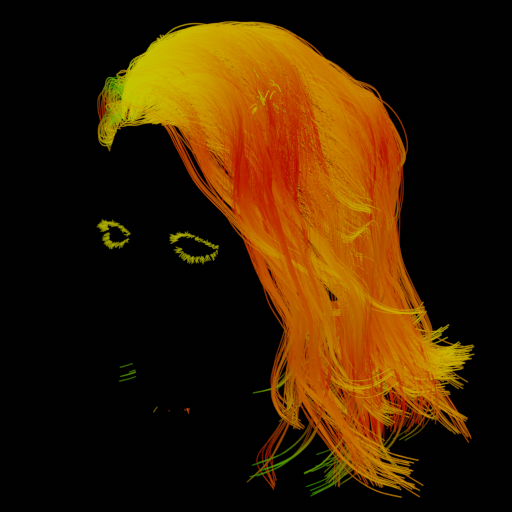
\includegraphics[width=0.2\textwidth]{project-final-paper/images/dataset/0009_hairdir.png}
    
        \caption{Synthetic dataset rendered by Blender}
        \label{fig:dataset}
    \end{figure}    

  \end{block}

  \begin{alertblock}{The Neural Orientation Field (NeOF) Model}

    The neural orientation field (NeOF) model we propose consists of multiple MLP layers and residual connections.
    
    \begin{itemize}
      \item \textbf{Input} Spatial coordinates $(x, y, z)$ of the point to be sampled
      \item \textbf{Output} World space hair orientation $(\theta, \phi)$, and opacity parameter $\sigma = (\sigma_{hair}, \sigma_{body})$
    \end{itemize}

  \end{alertblock}

  \begin{alertblock}{Volumetric Rendering for Neural Orientation Field}
  
    We propose a differentiable volumetric renderer to render both screen-space hair orientation, body/hair masks, and occupancy.
    
    To sample a pixel, we emit a camera ray with the known camera intrinsics and extrinsics on the filming plane. (Figure~\ref{fig:volumetric-renderer}) Then, the world space hair orientation and occupancy can be sampled along the camera ray. The volumetric rendering pipeline first projects the world space orientation to screen space, then integrate the screen space orientation with the sampled occupancy.

    \begin{figure}
        \centering
        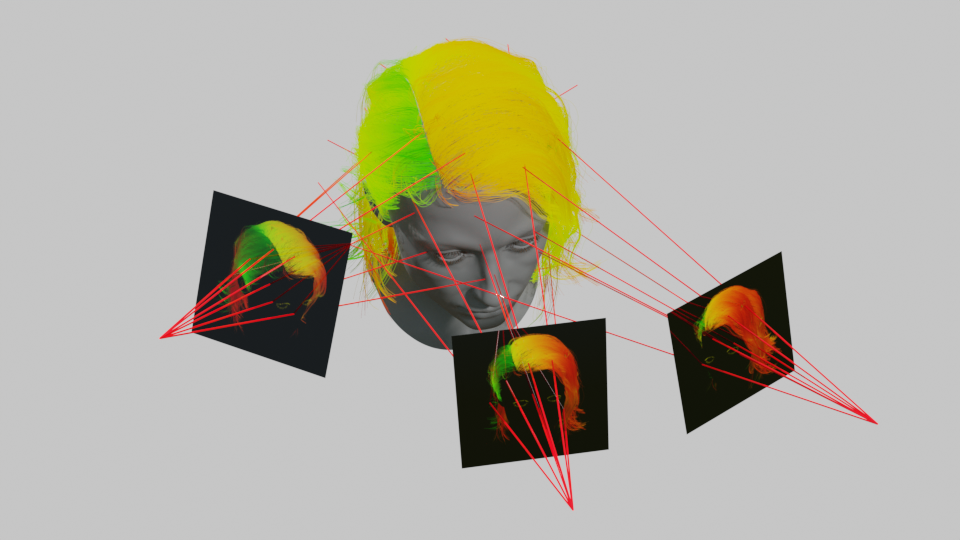
\includegraphics[width=0.6\linewidth]{project-final-paper/images/volumetric-renderer/volumetric-renderer.png}
        \caption{Volumetric Renderer}
        \label{fig:volumetric-renderer}
    \end{figure}
    
  \end{alertblock}

\end{column}

\separatorcolumn

\begin{column}{\colwidth}

  \begin{alertblock}{Volumetric Rendering for Neural Orientation Field}
    
    To project hair orientation, we first need to convert the world space orientation $\mathbf{o}_{world}$ to an orientation vector in homogeneous coordinate $\mathbf{v}_{world} \in \mathbb{R}^{4}$. Given the camera extrinsic matrix $M \in \mathbb{R}^{4 \times 4}$, $\mathbf{v}_{world}$ can be projected to the view space by $\mathbf{v}_{view} = M\mathbf{v}_{world}$.
    
    Normally, to project a world space vector onto screen space, we need to first apply view transform to get view space projection, then apply perspective transform to get screen space projection. However, as we choose pinhole camera as our camera model, the screen space orientation vectors are independent of the camera intrinsics. In other words, $\mathbf{v}_{screen} = \mathbf{v}_{view} = M\mathbf{v}_{world}$.
    
    Similar to the volumetric rendering function defined in NeRF \cite{mildenhall_nerf_2020}, our rendering function for screen space orientation can be written as:
    \begin{align}
    	V(\mathbf{r}) & = \int_{t_{n}}^{t_{f}} T(t) \sigma_{hair}(\mathbf{r}(t)) M \mathbf{v}_{world}(\mathbf{r}(t)) dt \\
    	T(t) & = exp(-\int_{t_{n}}^{t} \sigma_{body}(\mathbf{r}(s)) ds)
    \end{align}
    
    One important difference between our model and NeRF is we use two separate occupancy for body and hair, while in NeRF only one occupancy is used to integrate camera rays. In our case, camera rays can be blocked by face and body that doesn't contribute to the final integration. Therefore, we use $\sigma_{body}$ instead of $\sigma_{hair}$ to integrate residual ray $T(t)$.
    
    As we provide body mask and hair mask in the training data, we can also use the following rendering function to render body mask $B(\mathbf{r})$ and hair mask $H(\mathbf{r})$:
    \begin{align}
    	B(\mathbf{r}) & = 1 - exp(-\int_{t_{n}}^{t_{f}} \sigma_{body}(\mathbf{r}(s)) ds) \\
    	H(\mathbf{r}) & = 1 - exp(-\int_{t_{n}}^{t_{f}} \sigma_{hair}(\mathbf{r}(s)) ds)
    \end{align}
    
    Similar to the numerical estimation of radiance integration mentioned in NeRF, we use numerical estimation of orientation and mask integration defined as follows:
    \begin{align}
    	\hat{V}(\mathbf{r}) & = \sum_{i=1}^{N} T_{i} (1 - exp(-\sigma_{hair}^{(i)} \delta_{i})) M \mathbf{v}_{world}^{(i)} \\
    	T_{i} & = exp(-\sum_{j=1}^{i} \sigma_{body}^{(j)} \delta_{j}) \\
    	\hat{B}(\mathbf{r}) & = 1 - exp(-\sum_{i=1}^{N} \sigma_{body}^{(i)} \delta_{i}) \\
    	\hat{H}(\mathbf{r}) & = 1 - exp(-\sum_{i=1}^{N} \sigma_{hair}^{(i)} \delta_{i})
    \end{align}
    
    where $\delta_{i} = t_{i + 1} - t_{i}$. $\hat{V}(\mathbf{r})$, $\hat{B}(\mathbf{r})$, and $\hat{H}(\mathbf{r})$ are the final outputs of our volumetric render. The final loss is defined as the sum of orientation loss and mask losses. In theory, only orientation loss is required for the model to converge. However, we observed that introducing the mask losses helps improving the convergence speed. It also improves the model's performance on occupancy prediction accuracy.

  \end{alertblock}

\end{column}

\separatorcolumn

\begin{column}{\colwidth}

  \begin{block}{Result and Discussion}

    By comparing our method with the two baselines, HairStep \cite{zheng_hairstep_2023} and NeRF, we can observe from the evaluation metrics PSNR and MSE that our results outperform the two baselines. The result shows in Table \ref{tab:loss_comparison}. Sample images are shown in Figure \ref{fig:result_grid}. We represent the direction of planar hair at a given point using vectors formed by the red and green channels of the RGB images.
    
    \begin{table}[h]
    \centering
    \begin{tabular}{lccc}
    \toprule
    \textbf{Method} & \textbf{PSNR} & \textbf{MSE} \\ 
    \midrule
    NeOF (ours) & \textbf{15.06 dB} & \textbf{2026.75} \\
    HairStep & 13.97 dB & 2608.00 \\
    NeRF & 10.05 dB & 6429.77 \\
    \bottomrule
    \end{tabular}
    \caption{Comparison of losses between different methods}
    \label{tab:loss_comparison}
    \end{table}

    \begin{figure}[h]
        \centering
        
        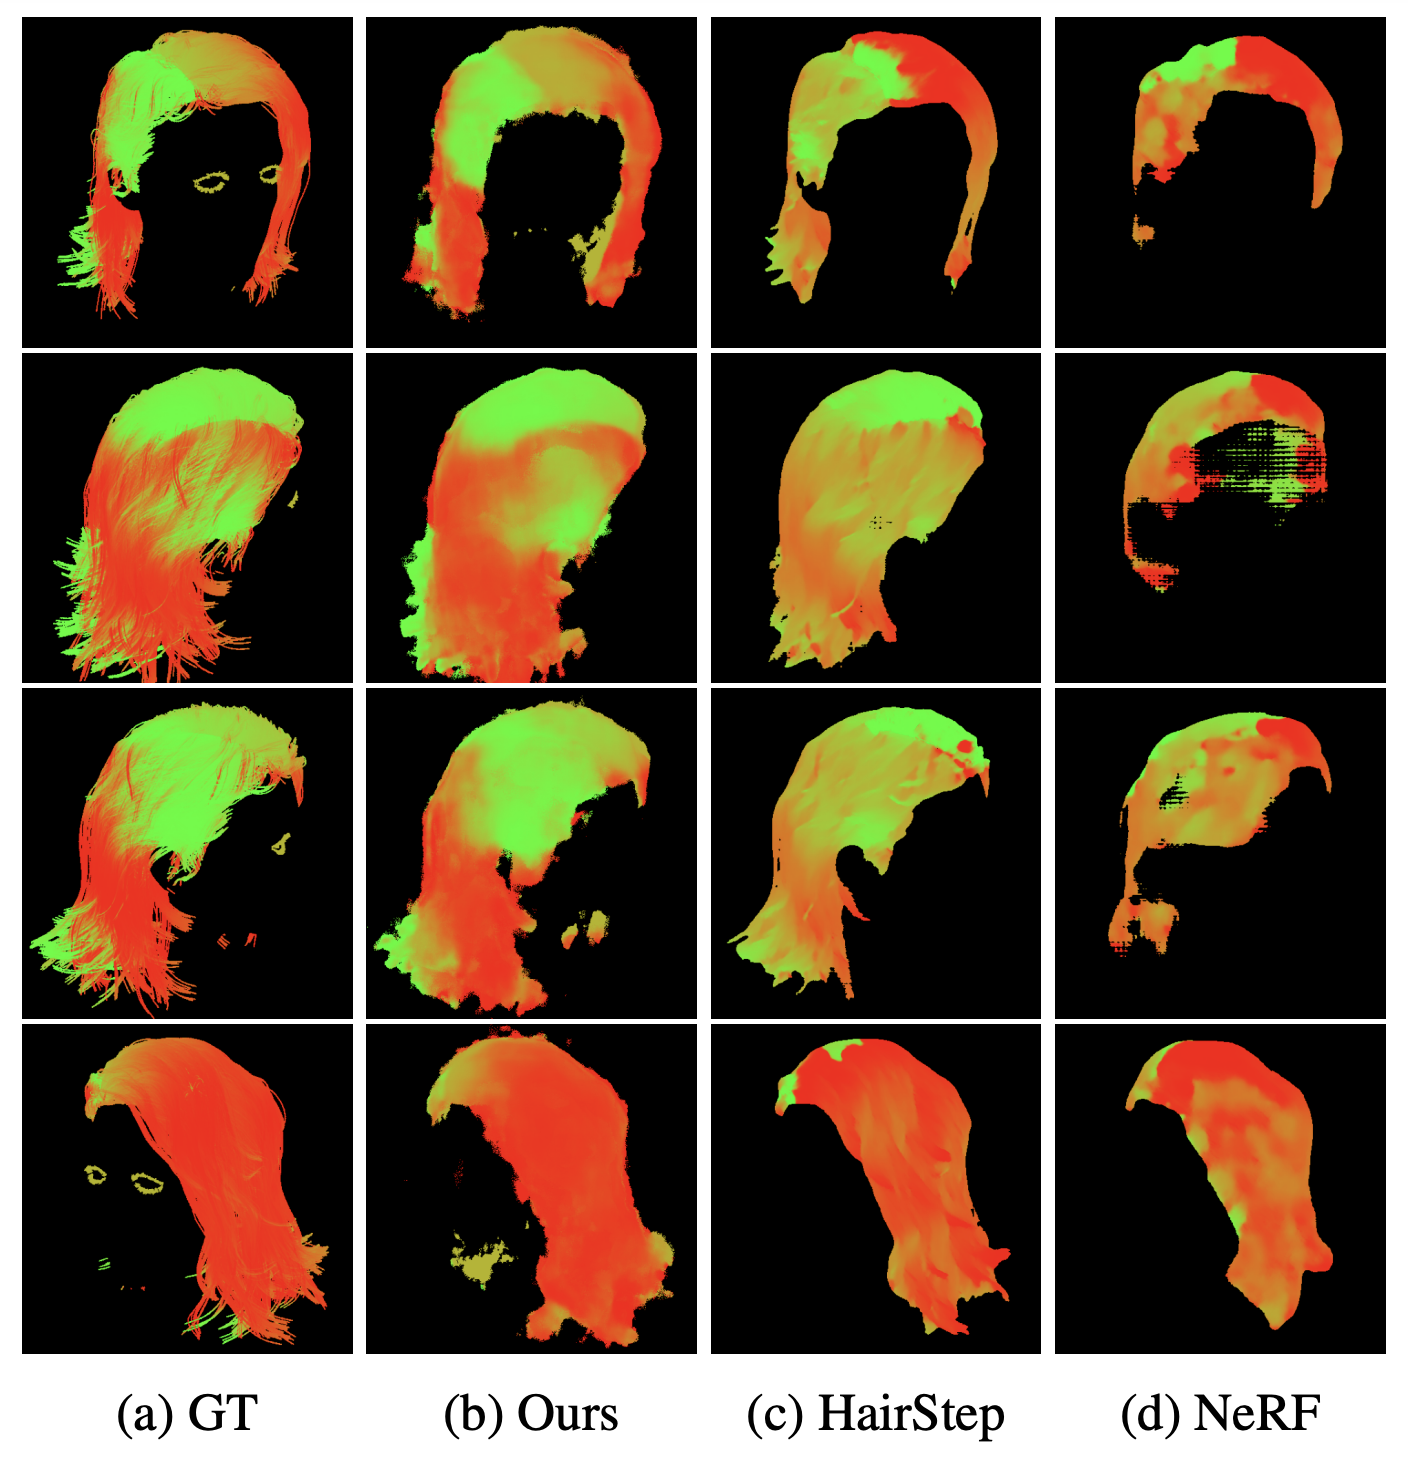
\includegraphics[width=0.6\linewidth]{poster/4by4.png}
        
        \caption{Normalized hair orientations, where (a) is the Ground Truth, (b) is the result our NeOF method, (c) is result of HairStep, and (d) is the result of traditional NeRF with HairStep.}
        \label{fig:result_grid}
    \end{figure}

    The overall vector field distribution of our method closely matches the ground truth. However, HairStep makes some errors when predicting some unintended horizontal components in areas where the hair extends vertically. This leads to discrepancies with the ground truth. For NeRF, the reconstructed 3D model is so blurry that hardly tells the strands apart, leading large errors in predicting the hair growth directions.

  \end{block}

  \begin{block}{Future}

  In the future, we aim to realize a complete 3D reconstruction pipeline, enabling our method to directly output editable 3D models compatible with Blender, facilitating further editing. We believe this approach will provide a straightforward and efficient solution for sampling and automating the modeling of real human hair, significantly reducing the costs associated with traditional hair modeling in the visual effects and animation industries.

  \end{block}

  \begin{block}{References}

    \nocite{*}
    \footnotesize{\bibliographystyle{plain}\bibliography{poster}}

  \end{block}

\end{column}

\separatorcolumn

\end{columns}

\end{frame}

\end{document}
